\documentclass[12pt]{article}
\usepackage{graphicx}

\newcommand{\imagespath}{../figures/us}

\begin{document}

\title{US All Communities Network Metrics Comparison Report}
\author{João Melga}
\date{\today}
\maketitle

Report with same graphs presented on the thesis for community 2 but now showing communities 0 and 1 as well. In addition, community 0 and 2 bipartite networks visualization (built with Gephi) were added.

\begin{figure}[htpb]
  \centering
  
\includegraphics[width=1\textwidth]{\imagespath/nestedness_evolution_all_communities_comparison.png}
  \caption{Nestedness evolution across all communities.}
  \label{fig:nestedness_evolution_all_communities_comparison}
\end{figure}

\begin{figure}[htpb]
  \centering
  
\includegraphics[width=1\textwidth]{\imagespath/network_metrics_evolution_all_communities.png}
  \caption{Network metrics evolution across all communities.}
  \label{fig:network_metrics_evolution_all_communities}
\end{figure}

\begin{figure}[htpb]
  \centering
  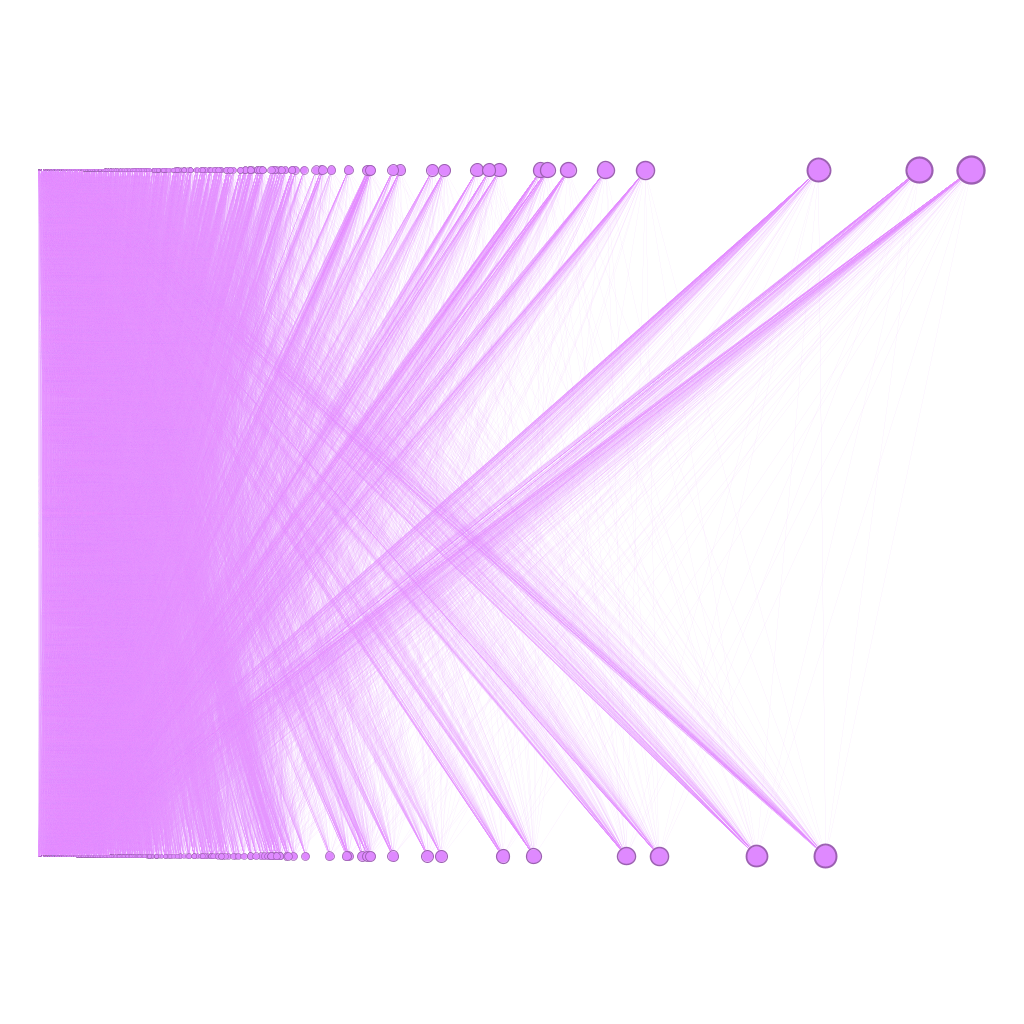
\includegraphics[width=1\textwidth]{../figures/gephi/us_comm_0_all_bipartite.png}
  \caption{Community 0 - All bipartite network visualization.}
  \label{fig:us_comm_0_all_bipartite}
\end{figure}

\begin{figure}[htpb]
  \centering
  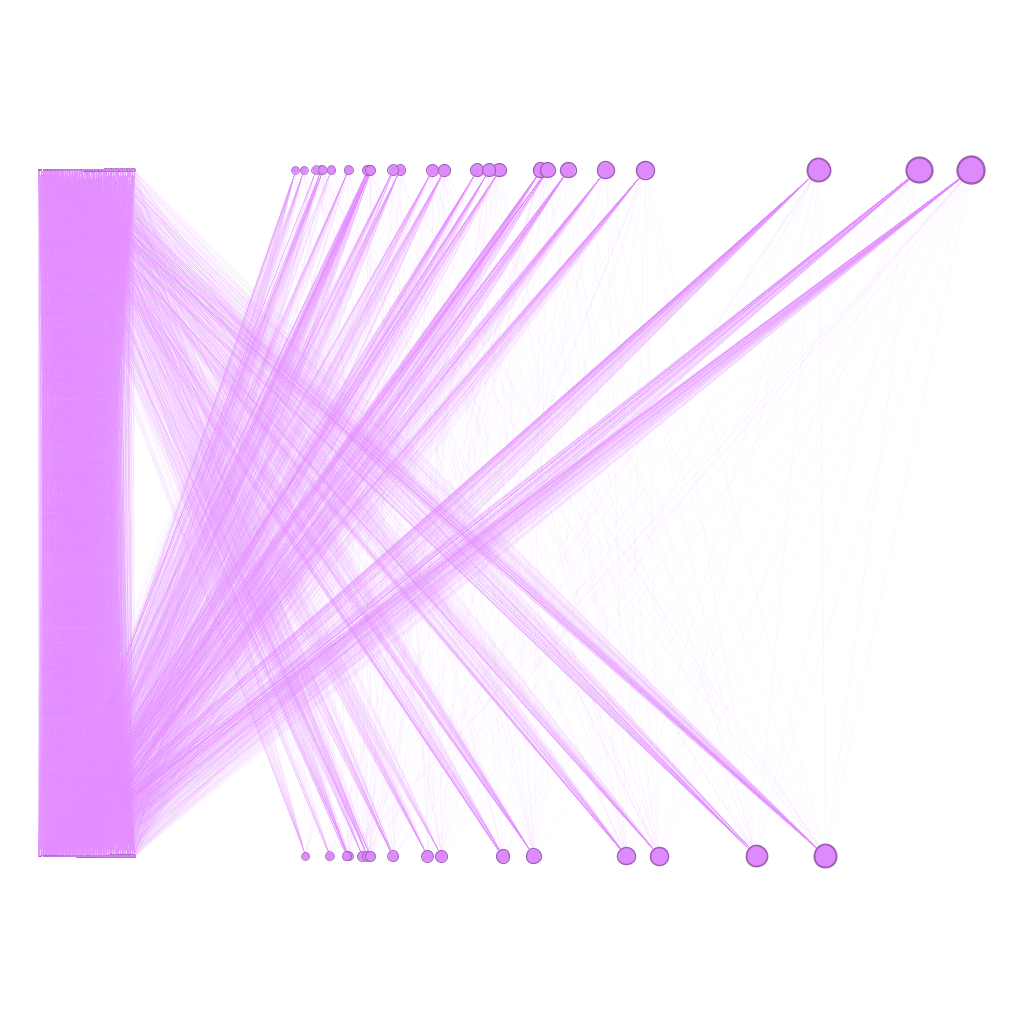
\includegraphics[width=1\textwidth]{../figures/gephi/us_comm_0_percentil_bipartite.png}
  \caption{Community 0 - Percentile bipartite network visualization.}
  \label{fig:us_comm_0_percentil_bipartite}
\end{figure}

\begin{figure}[htpb]
  \centering
  
\includegraphics[width=1\textwidth]{../figures/gephi/us_comm_2_all_bipartite.png}
  \caption{Community 2 - All bipartite network visualization.}
  \label{fig:us_comm_2_all_bipartite}
\end{figure}

\begin{figure}[htpb]
  \centering
  
\includegraphics[width=1\textwidth]{../figures/gephi/us_comm_2_percentil_bipartite.png}
  \caption{Community 2 - Percentile bipartite network visualization.}
  \label{fig:us_comm_2_percentil_bipartite}
\end{figure}

\end{document}